
%% ------------------------------------------------------------------------- %%
\chapter{Hash Tables}
\label{cap:Hash Tables}

%% ------------------------------------------------------------------- %%
%\begin{itemize}
%\item Define hash table and its operations
%\item Open Addressing Strategies (Linear Probing, Quadratic Probing, ...)
%\item Chaining Strategy (Simple Chaining, Move-to-front ...)
%\item Load factor and resizing/rehashing the table
%\end{itemize}
%% ------------------------------------------------------------------- %%


Hash tables or hash maps is one of the most used applications of hash functions. It is actually so used in computer science that is almost impossible to talk about one without mentioning the other. This data structure consists in associating a \textit{key} to a \textit{value} in a table. That is, given a \textit{key}, it can retrieve the  \textit{value} for it.

It is one of the possible, and many times considered the best, implementations of a dictionary. It has to implement the \texttt{insert}, \texttt{find} and \texttt{remove} operations, that can be accessed from outside the dictionary. It usually implements a lot of other private methods. 

This data structure is usually considered very useful among software engineers and computer scientists, although it usually has a linear worst case cost for retrieving, inserting and deleting a key-value pair. That is because hash tables usually have a constant average cost for those operations.

Moreover, when talking about hash tables we have the problem of key collision, that is when two keys map to the same hash value. As we saw in the previous chapter, collisions are more common than not, so collision resolution is a critical problem. To solve that problem, we have several techniques that involve different trade-offs. Those techniques are usually divided into two main categories, open addressing and separate chaining. Other problem to consider regarding this data structure is when to resize the hash table, to minimize the chance of collision and the use o memory. For this last one we usually consider a load factor, \( \alpha \), that is the ratio of keys with the available slots in the table.

\newpage

Also, hash tables can be easily abstracted to hash sets, commonly used to store a set of elements and check whether an element is in the set. We can abstract hash sets to a hash table always with an empty value. Hash sets are one of the common ways to implement sets in programming languages, like unordered\_set from C++14.

It is also important to notice that hash tables have applications in different areas of computer science also, like compilers, caches and database indexing.


\begin{figure}[h!]
  \centering
  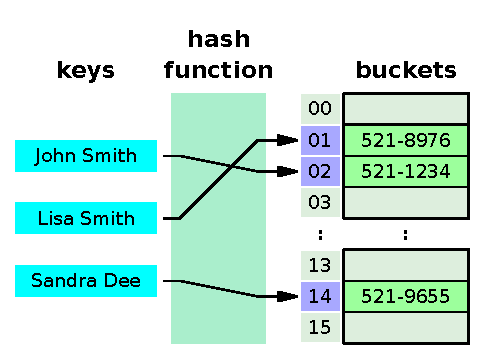
\includegraphics[width=12cm]{figuras/hash-table.pdf}
  \caption{Example of a hash table from string to string, more specifically name to phone number. Source: Wikipedia, Jorge Stolfi }
  \label{fig:hashTable}
\end{figure}

In the above figure (\ref{fig:hashTable}), we can see an example of a hash function that matches names of people to phone numbers, as we saw in the first chapter. This table has no collisions, and we can see that, for example, ``Jhon Smith'' has a hash value of 2 and his value in the table is ``521-1234''. That is we associated a names with phone numbers.

\newpage

\section{No collision open addressing hash table }

To start let's give an example of a hash table that has a perfect hash function, that is a function from \( X \) to \( [0, M) \) with no collisions from the used keys. For that example we use open addressing, that basically means that all data will be contained in an array (that is, the whole table). The operations \texttt{insert}, \texttt{find} and \texttt{remove} would be very easy to implement. For the sake of simplicity, we will assume all the keys are strings and values are integers. To start lets look at this simple class with dummy methods:

\begin{lstlisting}
class HashTable {
   vector< pair<string, int> > table;
   int m, n;
   
   HashTable() {
      m = 16;
      table.resize(m);
      n = 0;
   }

   unsigned int hashFunction(string s) {}
   
   void insert(string key, int value) {}

   int find(string key) {}

   void remove(string key) {}

private:
   double alpha = 1;
   void resizeIfNecessary() {}
}
\end{lstlisting}

As we can see it is pretty simple. The constructor builds a table of size \( 16 \), and we can assume a dynamic resizing every time the table is full. Later on we will see that this means that we resize every time the load factor, \( \alpha \), is equal to \( 1.00 \). We also can note that at the table part we are storing a pair of key and value, not just value. This is because we may want to retrieve all pairs of the table (like in a regular dictionary). The pairs are usually unordered (If they are not ordered by chance \dots). Actually, if one needs the set of keys sorted by total order, very likely hash tables are not the appropriate data structure. We will skip the implementation of hashFunction, as we already saw plenty of it in the last chapter, so we will go right in for the implementation of \texttt{insert}:

\begin{lstlisting}
void insert(string key, int value) {
  resizeIfNecessary();
  unsigned int idx = hashFunction(key);
  table[idx] = pair<string, int>(key, value);
  n++;
}
\end{lstlisting}

That is pretty simple, that is mostly because we will assume that we will never have a collision, so we just put the key on the position returned by the hash function. The method \texttt{find} is implemented as following:

\begin{lstlisting}
int find(string key) {
  unsigned int idx = hashFunction(key);
  if (table[idx].first == key)
    return table[idx].second;
  return 0;
}
\end{lstlisting}

Also very simple, we always know the value will be in position returned by idx. The \texttt{remove} will be of the same simplicity, as following:

\begin{lstlisting}
void remove(string key) {
  unsigned int idx = hashFunction(key);
  table[idx].first = pair<string, int>("", 0);
  n--;
}
\end{lstlisting}

Here we make the assumption that an empty position has an empty string. We could also carry a boolean, usually called a tombstone, to check if the position is occupied or not. If the hash function is perfect, than the insert, find and delete operations can be performed in constant time and linear space.

\section{Open addressing}

We can define open addressing in a general way as a hash table algorithm where the data always stay within the same vector. So, in the case of a collision, we need to define a systematic way to traverse the table. The sequence of elements we need to traverse when we have a collision is called \textit{``Probe sequence''}. With that our hash function would change to the following:
\[ h(x, i) \],
where \( x \) is our key and \( i \) is the probe sequence number. So every time we have a collision in \( h(x, i) \) we can simply go to \( h(x, i + 1) \). Given that, lets look into some different probe sequences.

\section{Linear Probing}

Linear probing is one of the most simple an practical probe sequences known. The probe sequence is basically:
\[ h(x, i) = (H(x) + i) ~\mathrm{mod}~ M \],
where \( M \) is the table size. That is a very simple probe sequence with not much secret on it. To implement the \texttt{insert} we can do the following:

\begin{lstlisting}
void insert(string key, int value) {
  resizeIfNecessary();
  unsigned int idx = hashFunction(key);
  while (table[idx] != pair<string, int>("", 0))
    idx = (idx + 1) % m;      
  table[idx] = pair<string, int>(key, value);
  n++;
}
\end{lstlisting}

That assumes that \texttt{pair<string, int>("", 0)} is the empty position, and performs a linear search until it finds one empty position to put the new (key, value) pair. The implementation of \texttt{find} is very similar:

\newpage

\begin{lstlisting}
int find(string key) {
  unsigned int idx = hashFunction(key);
  while (table[idx] != pair<string, int>("", 0)) {
    if (table[idx].first == key) 
      return table[idx].second;
    idx = (idx + 1) % m;
  }
  return 0; // Default value
}
\end{lstlisting}

It performs a linear search until it finds the element. If the key is not found the function returns a default value, that in our case is 0. 

For removal, we have the problem that we cannot leave ``holes'' in our table. That will be discussed more in depth later on the section ``How to delete an entry''. For now we will remove the element, and reinsert the key-value pairs that come right after it:

\begin{lstlisting}
void remove(string key) {
  unsigned int idx = hashFunction(key);
  while (table[idx] != pair<string, int>("", 0)) {
    if (table[idx].first == key) 
      break;
      idx = (idx + 1) % m;
  }
    
  if (table[idx].first == key) {
    table[idx] = pair<string, int>("", 0);
    vector< pair<string, int> > toRehash;
    int j = (idx + 1) % m;
    while (table[j] != pair<string, int>("", 0)) {
      toRehash.push_back(table[j]);
      table[j] = pair<string, int>("", 0);
      j = (j + 1) % m;
    }
    for (auto p : toRehash) {
      insert(p.first, p.second);
    }
    n--;
  }  
}
\end{lstlisting}

With that, the three operations have linear time complexity in the worst case. As we saw, we know hash functions that are considered good, with a rate of collision very close to an uniformly random function. Those functions will leave us with an expected constant time complexity for those operations, and we will see later on that in practice it is much faster than linear access. Another great benefit that linear probing has, specially when compared to other collision resolution strategies, is locality and cache friendliness.

However linear probing has the problem of clustering, that is long chains of occupied positions. This generates a greater problem, as long chains are only expected to get longer and longer. This can get worse if the hash function is not too sensitive to changes, having a lot of sequential hash values. 

\section{Quadratic Probing}

Another strategy for resolving collisions is quadratic probing. In this case, the probe sequence can be defined as:
\[ h(x, i) = (H(x) + i^2) \mod M \]
That solves the problem of having sequential hash values. The implementation of quadratic probing is very similar to the implementation of linear probing, with the exception that instead of adding one for each step we can keep the initial value and add the square of a counter.

However, quadratic probing doesn't solve the problem of clustering. Long chains are still expected to get longer and longer, the only difference is that the positions that lead to a longer chain are better distributed in the table. Another thing to notice is that quadratic probing has a worse locality and cache friendliness than linear probing. 

\section{Double Hashing}

As we saw the two strategies above have the problem of clustering, due to the fact that the sequences are the same for all keys. For that reason double hashing is a very good approach for open addressing. Double hashing probe sequence can be defined as following:
\[ h(x, i) = (H_1(x) + i * H_2(x)) \mod M \],
where \( H_1 \) and \( H_2 \) are two distinct hash functions. In that way not only the initial hash value will depend on \( x \), but it's probe sequence offset (that is, the number of slots between \(h(x, i) \) and \(h(x, i + 1) \)) will too. The implementation of double hashing is very similar to both quadratic and linear probing, except that we sum a different offset.

These last three implementations of hash table give us linear time worst case complexity for all operations and constant time expected time complexity under the simple uniform hashing assumption.

\section{Robin Hood Hashing}

Robin Hood Hashing is an optimization technique regarding collision resolution with open addressing. It should be paired with Linear Probing, Quadratic Probing or Double Hashing, but usually it is paired with linear probing due to it is good locality and cache friendliness. It is basic is that it minimizes the distance of each key from its ``home Slot'', that is, its initial hash value position. \citep{RobinHoodHashing}. Also, Robin Hood hashing is one of the few open addressing strategies to be built-in in hash tables of some languages, such as Rust.

In order to minimize the distance from each key from its home slot, Robin Hood hashing uses a concept that is called Probe Sequence Length, or PSL, of a key-value pair. The PSL of a key-value pair is the number of probes required to find that pair. For that reason we need to define a new class to store in our table, that we will call \texttt{Node}:

\begin{lstlisting}
class Node {
public:
   string key;
   int value;
   unsigned int PSL;   
   Node(string K = "", int V = 0, unsigned int P = 0):
      key(K), value(V), PSL(P) {}

   bool operator == (const Node& ot) {
      return key == ot.key && value == ot.value && PSL == ot.PSL;
   }
   bool operator != (const Node& ot) {
      return key != ot.key || value != ot.value || PSL != ot.PSL;
   }
};

const Node defaultNode = Node();
\end{lstlisting}

\texttt{Node} is a very simple class that stores a key, a value and an unsigned integer that is the PSL. The main idea around Robin Hood hashing it to move the Nodes with a low PSL in favor of Nodes with a high PSL. We can think of Nodes with a high PSL as poor, because we take longer to find it, and Nodes with a low PSL as rich because we can find them faster. For that reason the algorithm is called Robin Hood Hashing \citep{RobinHoodHashing}.

As explained when inserting an element we first look for an empty position. While searching for it, we check whether the \texttt{Node} that is in the way has a lower PSL than the Node that we are inserting, and if that is the case we swap them, securing a position for the current Node and move the other node forward. The implementation of this algorithm using Linear Probing would be the following:

\begin{lstlisting}
void insert(string key, int value) {
  resizeIfNecessary();
  unsigned int idx = hashFunction(key);
  Node toInsert = Node(key, value, 0);
  while (table[idx] != defaultNode) {
    if (toInsert.PSL > table[idx].PSL)
      swap(toInsert, table[idx]);         
    idx = (idx + 1) % m;
    toInsert.PSL++;
  }
  table[idx] = toInsert;
  n++;
}
\end{lstlisting}

For the \texttt{find} method we can use different lookup techniques. Here we will focus on the lookup that is most similar with linear probing, but with a tweak that will make finding that keys are not present faster. While searching for a key, we can calculate what the PSL of that key would be if were inserted, and if we find a Node with a greater PSL that means the pair is not present. That is because all Nodes after it will also have a PSL greater than the current PSL. The implementation of what was described above would be the following:

\newpage

\begin{lstlisting}
int find(string key) {
  unsigned int idx = hashFunction(key);
  unsigned int curPSL = 0;
  while (table[idx] != defaultNode) {
    if (table[idx].key == key) 
      return table[idx].value;
    // If the key were inserted it would be before this Node.
    if (table[idx].PSL > curPSL)
      break; 
    idx = (idx + 1) % m;
    curPSL++;
  }
  return 0; // Default value
}
\end{lstlisting}

For the removal we can apply \textit{backward shifting}. Although this will be discussed more in depth in the ``How to delete an entry'' section, this approach is unique to robin hood hashing and has a better performance than rehashing.

\textit{Backward shifting} consists in first clearing out the slot that contains the key to be removed, then shifting the following keys one step back until a Node with 0 PSL or an empty slot is encountered. The code for that would be the following:

\begin{lstlisting}
void remove(string key) {
  unsigned int idx = hashFunction(key);
  while (table[idx] != defaultNode) {
    if (table[idx].key == key) 
      break;
    idx = (idx + 1) % m;
  }
  if (table[idx].key == key) {
    table[idx] = defaultNode;
    while (table[(idx + 1) % m] != defaultNode &&
           table[(idx + 1) % m].PSL != 0) {
      swap(table[idx], table[(idx + 1) % m]);
      table[idx].PSL--;
      idx = (idx + 1) % m;
    }
    n--;
  }
}
\end{lstlisting}

We can always do that because the keys are always sorted according to the their home slot (That is, the first Node with PSL that is 0 that comes before them).

The worst time complexity of all operations is linear and the expected time complexity is constant. The expected length of the longest PSL in a full table is \( \log n \).
\section{Cuckoo Hashing}

Another well known strategy for collision resolution in open addressing is Cuckoo Hashing. It is a different strategy regarding the previous ones because it uses more than one array, usually two, but up to any number of arrays, to perform collision resolution. It is usually classified as open addressing because each slot can hold up to one key-value pair. For this explanation let's assume that we are using two arrays. Cuckoo hashing requires also one hash function per array used, in our case two hash functions.

%% Image representing cuckoo hashing

For the insertion of cuckoo hashing we try to insert the key in the first table and if a collision occurs we swap the key value pair that we are trying to insert with the element that is currently on the table and then try to insert it on the next array. If a collision occurs in the other array we swap the pairs and try again on the next one, until we find an empty position or we reach a certain threshold. The threshold is important because we can have cycles.

%% Image Representing insertion.

The code for the algorithm described above is the following:

\begin{lstlisting}
void insert(string key, int value) {
  resizeIfNecessary();
  unsigned int j = 0, it = 0;
  unsigned int idx = hashFunction(key, j), lim = maxLoop();
  pair<string, int> toInsert = pair<string, int>(key, value);
  while (table[j][idx] != pair<string, int>("", 0) && it < lim) {
    swap(table[j][idx], toInsert);
    j = (j + 1) % numTables;
    idx = hashFunction(toInsert.first, j);
    it++;
  }
  if (it == lim)
    resize();
  table[j][idx] = toInsert;
  n++;
}
\end{lstlisting}

This gives a very strong property to this collision resolution approach, that is every key value pair will be in its corresponding position in exactly one of the arrays. And this will give constant Lookup and Removal time. 

In order to find a key value pair we just need to look if the key value pair is present in one of the tables. The code is the following:

\begin{lstlisting}
int find(string key) {
  for (unsigned int j = 0; j < numTables; j++) {
    unsigned int idx = hashFunction(key, j);
    if (table[j][idx].first == key)
      return table[j][idx].second;
  }
  return 0;
}
\end{lstlisting}

For removal we can simply erase the key value pair from the table, as no key value pair affect the lookup of any other pair. The code is the following:

\begin{lstlisting}
void remove(string key) {
  for (unsigned int j = 0; j < numTables; j++) {
    unsigned int idx = hashFunction(key, j);
    if (table[j][idx].first == key) {
      table[j][idx] = pair<string, int>("", 0);
      n--;
    }
  }
}
\end{lstlisting}

Besides the amazing property of guaranteed constant lookup and removal, Cuckoo hashing has the problem of cycles during insertion, which can cause unwanted rehashes. To deal with that, many implementations also use a stash to keep a constant amount of elements in case the threshold is reached. A stash is a sort of ``bin'' of fixed size that we put key-value pairs that failed insertion, and during lookup we would also need to look at the stash.

\section{Coalesced Hashing}

Another well known strategy, described in Donald Knuth book \citep{TAOCP3}, is Coalesced Hashing. Although without much advantages in contrast with previous strategies, coalesced hashing condenses the hash table well in memory and is very similar to Chaining Hashing, our next topic.

The main idea of coalesced hashing is to add a new parameter to our key value pairs in the table, called next. That would create linked lists in the table in case we have a collision. To find the next element in case a collision we can find the first free bucket looking to the array in reverse order. The function to find the next free bucket is the following:

\begin{lstlisting}
int nextFreeBucket() {
  for (int i = m - 1; i >= 0; i--) {
    if (table[i].isDefaultNode())
      return (unsigned int)i;
    }
  return -1; // error
}
\end{lstlisting}

To insert an element, in case of a collision, we need to traverse the linked list beginning on the bucket that the key hashes to until the end. Then we add a new Node to the end of the linked list, pointing to the next free bucket. The complete code of the insertion algorithm will be shown later on.

To lookup for an element, we can traverse the linked list until we find a matching Node. The code for the find method would be the following:

\begin{lstlisting}
int find(string key) {
  unsigned int idx = hashFunction(key);
  while (idx != -1) {
    if (table[idx].key == key) 
      return table[idx].value;
    idx = table[idx].next;         
  }    
  return 0;
}
\end{lstlisting}

Removing a node in coalesced hashing is very difficult, as many other nodes can depend on it. For this reason the best way to delete an element in coalesced hashing is by using a strategy that is known as tombstoning. The idea of this strategy is to put a placeholder value, that will be considered as occupied by the find method but as free by the insertion method. The code for that would be the following:

\begin{lstlisting}
void remove(string key) {
  unsigned int idx = hashFunction(key);
  while (idx != -1) {
    if (table[idx].key == key) 
      break;
    idx = table[idx].next;         
  }
  if (table[idx].key == key) {
    table[idx].transformTombstone();
    n--;
  }
}
\end{lstlisting}

For this reason, the insertion method explained earlier on would have to be a little bit different, considering tombstones. The code would look like the following:

\begin{lstlisting}
void insert(string key, int value) {
  resizeIfNecessary();
  unsigned int idx = hashFunction(key);
  Node toInsert = Node(key, value, -1);
  if (!table[idx].isDefaultNode()) {
    while (table[idx].next != -1 && !table[idx].isTombstone())
      idx = table[idx].next; 
    if (!table[idx].isTombstone()) {
      table[idx].next = nextFreeBucket();
      idx = table[idx].next;
    }
  }
  table[idx] = toInsert;
  n++;
}
\end{lstlisting}

\section{Chaining hashing}

Chaining hashing, also known as closed addressing, is the implementation of a hash table using a container, usually called bucket, to store the (key, value) pairs with a given hash. On this implementation, each bucket of the table is a linked list, that will carry the key value pair in our case. We deal with collisions with this implementation by adding a new node to the start of the list.

This implementation is considered simpler than open addressing, usually because the way of dealing with collisions is clearer. Also it is less system dependent if we consider performance (as we saw one of the key advantages of open addressing is that it is cache friendly). That is one of the key reasons that C++ uses chaining hashing for its default implementation of unordered\_hash \citep{HashTableProposal}.

Below we will discuss an implementation of chaining hashing.

\section{Simple Chaining Hashing Algorithm}

For this chaining hashing implementation we will use C++14 STL data structure list as our container. list is a doubly linked list. For our \texttt{insert} we can implement it in the following way:

\begin{lstlisting}
void insert(string key, int value) {
  resizeIfNecessary();
  unsigned int idx = hashFunction(key);      
  table[idx].emplace_front(key, value);
  n++;
}
\end{lstlisting}

As we can see it is a very simple implementation, we just push a new element in the front of the list pointed in the idx. As before we add the counter of elements in the list and call resizeIfNcessary().

For \texttt{find} we can implement in the following way:

\begin{lstlisting}
int find(string key) {
  unsigned int idx = hashFunction(key);
  auto it = find_if(table[idx].begin(), table[idx].end(),
                    [&key](auto& kv) { return kv.first == key; });
  if (it != table[idx].end())
    return it->second;
  return 0;
}
\end{lstlisting}

That implementation is very succinct but uses some of the features of C++14 (such as generic lambdas). For \texttt{erase} we can implement in a very similar fashion:

\begin{lstlisting}
void remove(string key) {
  unsigned int idx = hashFunction(key);
  auto it = find_if(table[idx].begin(), table[idx].end(),
                    [&key](auto& kv) { return kv.first == key; });
  if (it != table[idx].end()) {
    table[idx].erase(it);
    n--;
  }
}
\end{lstlisting}

As we can see, with linked list it is clearly easier to erase an element. 

The naive algorithm of chaining hashing with a linked list gives linear worst time complexity for all operations and constant expected time complexity under the assumption of simple uniform hashing. 

% THINK ABOUT PUTTING THAT.

%One interesting thing to notice regarding chaining hashing implementation in C++ is that we may have a greater performance with implementations using vector instead of list, because of the better locality of vector.

\section{Move to front}

One great optimization to chaining hashing is every time you execute the \texttt{find} method to move to the beginning of the container the element that was found. That will keep in the beginning of the container the elements that are searched the most. As in many applications we can apply the 80 / 20 rule this greatly helps in time performance. The 80 / 20 rule is basically the idea that usually, 20\% of the keys will represent 80\% of the searches, this rule is also cited by Knuth \citep{TAOCP3}.

If our container is a linked list we can easily adapt the above implementation to move to front every time we search an element, with const time complexity cost. The implementation of \texttt{find} would be the following:

\begin{lstlisting}
int find(string key) {
  unsigned int idx = hashFunction(key);
  auto it = find_if(table[idx].begin(), table[idx].end(),
                    [&key](auto& kv) { return kv.first == key; });
  if (it != table[idx].end()) {
    if (it != table[idx].begin()) {
      table[idx].splice(table[idx].begin(), table[idx],
                        it, next(it));
    }
    return it->second;
  }
  return 0;
}
\end{lstlisting}

Here we are using the \texttt{splice} method of list C++ standard library to move an element inside a list. This still keeps the complexity of \texttt{find} in linear worst time and constant expected time. It is important to notice here that if our container wasn't a linked list we could take longer than constant time to move it to front.


\section{How to delete an entry}

In open addressing deleting an entry is considered hard by many of the collision resolution methods. Between clearing the entry and rehashing, clearing the entry and shifting the elements back or using tombstone, tombstone is usually considered the fastest approach due to its laziness.
The problem with tombstones is that it can make the table ``dirty'' if we have a high number of deletions, making lookups or insertions slower. So one suggestion is to rehash your table in the case of a high number of tombstones.

In contrast, deleting an entry in chaining hashing is delegated to the container that contains the key. That is, if we have a linked list as our container we just delegate the deletion to it. This is much easier is create less problems than open addressing deletion. That is one of the reasons why chaining hashing is usually chosen for default hash table implementation in many languages, like in C++ \citep{UnorderedMapDiscussion}.

\section{When to resize an array}

In open addressing the load factor to resize a hash table can't be greater than 1.0, because the table can't have more elements than its capacity. That is not true for chaining hashing as we will see later on. A good load factor depends on several factors, such as the strategy used. Some strategies are more ``permissive'' of a load factor closer to 1, Robin Hood for example can still work well with load factors close to 0.9 and doesn't lose much performance with load factors greater than that \citep{RobinHoodDefault}. On the other hand, Cuckoo Hashing doesn't work well with load factors greater than 0.5. Higher load factors means a better use o memory, which is an advantage of Open Addressing, where lower load factors means more memory used but greater efficiency when using the data structure. For that reason we try to always use the greater load factor possible without degrading much performance when using open addressing. In general this value ranges from 0.3 for cuckoo hashing up to .9 for Robin Hood hashing.

In contrast to open addressing, chaining hashing can have max load factors greater than 1.0, although many times those are not used, and when they are used they are not far from 1.0. Default hash tables of C++ and Java use chaining hashing, and the max load factor for a hash table in C++ is 1.0, while for java is 0.75. \citep{MaxLoadFactorCplusplus}.
It can be easily proven that the expected time complexity for operations in chaining hashing is \( O(1 + \alpha) \) where \( \alpha \) is the max load factor. For that reason an big alphas still works reasonably well with chaining hashing. Golang for example has 6.5 as max load factor.
Although chaining hashing can still work well with bigger load factors it ends up using more memory and also has a worse locality for cache purposes.

\section{Open Addressing vs Chaining Hashing}

When comparing Open Addressing vs Chaining hashing we can cite many pros and cons. Let us start with the open addressing pros. Among the pros of open addressing we can see that open addressing techniques such as linear probing tend to be more cache friendly. That is because as the key value pairs are stored in the memory in a sequential way with the vector, when loading a key value pair we will load a chunck of memory that is around it (that will have other key value pairs). Related to it is the 80 / 20 rule, that when applied to hash tables means that ``in practice'' 80\% of the keys will be accessed 20\% of the time (and 20\% of the keys will be accessed 80\% of the time). This is only for illustration purposes, obviously this is not valid for every application, as we can artificially create one that does not follow the rule. Another advantage of open addressing is that all the memory will be in a single and sequential ``Block'' of memory. 